\documentclass[letterpaper]{article} % DO NOT CHANGE THIS
\usepackage[submission]{aaai2027}  % DO NOT CHANGE THIS
% The serif, sans-serif, and monospaced fonts are loaded automatically by
% aaai2027.sty (newtxtext, helvet, courier). DO NOT add \usepackage{times},
% \usepackage{helvet}, \usepackage{courier}, or any other font package.
\usepackage[hyphens]{url}  % DO NOT CHANGE THIS
\usepackage{graphicx} % DO NOT CHANGE THIS
\urlstyle{rm} % DO NOT CHANGE THIS
\def\UrlFont{\rm}  % DO NOT CHANGE THIS
\usepackage{natbib}  % DO NOT CHANGE THIS AND DO NOT ADD ANY OPTIONS TO IT
\usepackage{caption} % DO NOT CHANGE THIS AND DO NOT ADD ANY OPTIONS TO IT
\frenchspacing  % DO NOT CHANGE THIS
%
% These are recommended to typeset algorithms but not required. See the subsubsection on algorithms. Remove them if you don't have algorithms in your paper.
\usepackage{algorithm}
\usepackage{algorithmic}

%
% These are recommended to typeset listings but not required. See the subsubsection on listing. Remove this block if you don't have listings in your paper.
\usepackage{newfloat}
\usepackage{listings}
\DeclareCaptionStyle{ruled}{labelfont=normalfont,labelsep=colon,strut=off} % DO NOT CHANGE THIS
\lstset{%
	basicstyle={\footnotesize\ttfamily},% footnotesize acceptable for monospace
	numbers=left,numberstyle=\footnotesize,xleftmargin=2em,% show line numbers, remove this entire line if you don't want the numbers.
	aboveskip=0pt,belowskip=0pt,%
	showstringspaces=false,tabsize=2,breaklines=true}
\floatstyle{ruled}
\newfloat{listing}{tb}{lst}{}
\floatname{listing}{Listing}

%
% Recommended for better-looking tables
\usepackage{booktabs}

%
% Keep the \pdfinfo as shown here. There's no need
% for you to add the /Title and /Author tags.
\pdfinfo{
/TemplateVersion (2027.1)
}

% DISALLOWED PACKAGES
% \usepackage{authblk} -- This package is specifically forbidden
% \usepackage{balance} -- This package is specifically forbidden
% \usepackage{CJK} -- This package is specifically forbidden
% \usepackage{float} -- This package is specifically forbidden
% \usepackage{flushend} -- This package is specifically forbidden
% \usepackage{fullpage} -- This package is specifically forbidden
% \usepackage{geometry} -- This package is specifically forbidden
% \usepackage{hyperref} -- This package is specifically forbidden
% \usepackage{navigator} -- This package is specifically forbidden
% (or any other package that embeds links such as navigator or hyperref)
% \usepackage{indentfirst} -- This package is specifically forbidden
% \usepackage{layout} -- This package is specifically forbidden
% \usepackage{multicol} -- This package is specifically forbidden
% \usepackage{nameref} -- This package is specifically forbidden
% \usepackage{savetrees} -- This package is specifically forbidden
% \usepackage{setspace} -- This package is specifically forbidden
% \usepackage{stfloats} -- This package is specifically forbidden
% \usepackage{tabu} -- This package is specifically forbidden
% \usepackage{titlesec} -- This package is specifically forbidden
% \usepackage{tocbibind} -- This package is specifically forbidden
% \usepackage{ulem} -- This package is specifically forbidden
% \usepackage{wrapfig} -- This package is specifically forbidden
% DISALLOWED COMMANDS
% \nocopyright -- Your paper will not be published if you use this command
% \addtolength -- This command may not be used
% \balance -- This command may not be used
% \baselinestretch -- Your paper will not be published if you use this command
% \clearpage -- No page breaks of any kind may be used for the final version of your paper
% \columnsep -- This command may not be used
% \newpage -- No page breaks of any kind may be used for the final version of your paper
% \pagebreak -- No page breaks of any kind may be used for the final version of your paper
% \pagestyle -- This command may not be used
% \small -- This is not an acceptable font size.
% \vspace{- -- No negative value may be used in proximity of a caption, figure, table, section, subsection, subsubsection, or reference
% \vskip{- -- No negative value may be used to alter spacing above or below a caption, figure, table, section, subsection, subsubsection, or reference

\usepackage{amsmath,amssymb}
\usepackage{xcolor}
\usepackage{multirow}
\usepackage{array}
\usepackage{enumitem}
\usepackage{subcaption}
\usepackage{tablefootnote}
\usepackage{colortbl}
\usepackage{pifont}  % for \ding symbols
\usepackage{tikz}
\usetikzlibrary{arrows.meta,positioning,fit,backgrounds,calc,decorations.pathreplacing,patterns,shapes.geometric}
\usepackage{tcolorbox}
\tcbuselibrary{skins,breakable}

% ── Color palette (NeurIPS-style, colorblind-friendly) ──
\definecolor{bestcolor}{HTML}{E8F5E9}
\definecolor{gaincolor}{HTML}{1B5E20}
\definecolor{cStandard}{HTML}{BF616A}   % muted red
\definecolor{cAOI}{HTML}{5E81AC}        % steel blue
\definecolor{cDelta}{HTML}{A3BE8C}      % sage green
\definecolor{cVisual}{HTML}{D08770}     % muted orange
\definecolor{cASR}{HTML}{B48EAD}        % muted purple
\definecolor{cNarr}{HTML}{88C0D0}       % light blue
\definecolor{cAccent}{HTML}{EBCB8B}     % warm yellow
\definecolor{cGray}{HTML}{4C566A}       % dark gray
\definecolor{cLightGray}{HTML}{D8DEE9}  % light gray

\setcounter{secnumdepth}{2} %May be changed to 1 or 2 if section numbers are desired.

% The file aaai2027.sty is the style file for AAAI Press
% proceedings, working notes, and technical reports.
%

% Title

% Your title must be in mixed case, not sentence case.
% That means all verbs (including short verbs like be, is, using,and go),
% nouns, adverbs, adjectives should be capitalized, including both words in hyphenated terms, while
% articles, conjunctions, and prepositions are lower case unless they
% directly follow a colon or long dash
\title{Agent-Computer Observation Interfaces\\Enable Dynamic Computer Use}
\author{
    %Authors
    % All authors must be in the same font size and format.
    Anonymous Submission
}
\affiliations{
    
}

\begin{document}

\maketitle

\begin{abstract}
SWE-agent~\citep{sweagent} established the \emph{action} interface as an underexplored design axis for software-engineering agents. We make the analogous case for the \emph{observation} interface in computer-use (CU) agents. Current CU agents observe the world through periodic screenshots (every 3--5\,s) with no audio, leaving them blind to dynamic content and deaf to speech.

We introduce the \textbf{Agent-Computer Observation Interface (AOI)}, a lightweight, model-agnostic perception layer that decouples continuous, adaptive observation from discrete actions. It has three gated components---inter-step keyframe capture, volume-gated audio transcription, and persistent model-generated visual narration---with almost zero overhead on static tasks.

On \textbf{DynaCU-Bench} (100 dynamic browser tasks plus a 50-task static control), eight CU models from 7B to frontier scale gain $+17$ to $+48$\,pp with zero retraining (paired McNemar $p<10^{-3}$ for all); Claude Sonnet~4.6 reaches 78.7\% (3-seed mean). AOI also outperforms production streaming baselines on audio tasks (12/12 vs.\ 3/12 and 0/12). Three findings reframe CU perception: keyframe value emerges primarily through narration; narration mainly helps models articulate what they see; and the observation interface is not a fixed bundle---its optimal composition is model-specific.
\end{abstract}

% Uncomment the following to link to your code, datasets, an extended version or similar.
% You must keep this block between (not within) the abstract and the main body of the paper.
% Make sure that you do not de-anonymize yourself with these links.
% \begin{links}
%     \link{Code}{https://github.com/19PINE-AI/AOI}
%     \link{Website}{https://01.me/research/AOI}
% \end{links}

% ════════════════════════════════════════════════════════════
\section{Introduction}
\label{sec:intro}
% ════════════════════════════════════════════════════════════

\textbf{Computer-use agents are blind between screenshots and deaf to audio.}
Current CU agents perceive the world through static screenshots every 3--5 seconds with no audio channel.
Between snapshots they miss videos, animations, and transient UI events. Furthermore, they have zero perception of meeting speeches, spoken instructions, or notification chimes.
Therefore, an entire class of everyday tasks---watching screencasts, following meetings, and responding to voice prompts---remains out of reach.

\textbf{The gap is real and unaddressed.}
While screenshot-based agents have reached over 50\% on static benchmarks like OSWorld~\citep{osworld,surfer2,uitars2}, dynamic and audio-heavy tasks lag far behind. Video models struggle on temporal reasoning~\citep{guiworld,videowebarena,videogamebench,cuasuite}, and even recent surveys overlook the observation modality itself~\citep{cusurvey}.

\textbf{The observation interface is a separable design axis.}
Improving perception via model retraining is expensive and model-specific. Inspired by SWE-agent~\citep{sweagent}, which advanced the field by redesigning the \emph{action} interface rather than the model, we argue that the \emph{observation} interface is the analogous lever. Prior work enriches \emph{what} a single screenshot contains, but leaves \emph{when} the agent looks and through which senses largely untouched.

Our core principle is \emph{decoupling continuous, adaptive, multimodal observation from discrete actions}.

\textbf{Our approach.}
We introduce the \textbf{Agent-Computer Observation Interface (AOI)}, a lightweight
perception layer placed between the environment and any image-based CU model.
AOI uses three gated components:
inter-step keyframe capture, volume-gated audio transcription, and
model-generated visual narration that persists as text. It has near-zero overhead on static tasks and no retraining is required. However, the optimal component mix is model-specific.

\textbf{Contributions.}
\begin{enumerate}
  \item We identify the \textbf{observation interface} as a separable CU design axis, complementary to SWE-agent's action interface, with \emph{decoupling observation from action} as the core principle.
  \item We introduce the \textbf{Agent-Computer Observation Interface (AOI)}, a model-agnostic perception layer with three gated components. We release AOI together with \textbf{DynaCU-Bench}, a benchmark of 100 dynamic tasks and a static task control set.
  \item AOI delivers significant gains across eight CU modelson dynamic tasks with zero retraining (Section~\ref{sec:eval}), without harming static work.
  \item We decompose the gains: keyframe value emerges mainly through narration, and the optimal component mix is model-specific (Sections~\ref{sec:analysis}--\ref{sec:newer}).
\end{enumerate}

% ════════════════════════════════════════════════════════════
\section{Background: The CU Agent Loop}
\label{sec:background}
% ════════════════════════════════════════════════════════════

Every current CU agent follows a fixed \emph{observe\,$\to$\,reason\,$\to$\,act}
cycle: capture a screenshot $s_t$, sample an action
$a_t$ conditioned on $s_t$ and trajectory history $\tau$, execute it, wait a short buffer $\delta$, and repeat.
Two spaces define an agent's capabilities.
The \textbf{action space} $\mathcal{A}$ is a small grammar of discrete commands---click, type, scroll,
wait, done---that has seen substantial prior innovation~\citep{sweagent}.
By contrast, the \textbf{observation space} $\mathcal{S}$ remains severely limited to a single RGB screenshot per step.

This design leaves agents blind between screenshots. The typical 3--5 second interval means motion, and transient UI events are almost entirely missed. Furthermore, the lack of an audio channel leaves agents deaf to all sounds.
Concretely, four categories of content are systematically missed:
(i)~\emph{transient events}---toasts and dialogs that appear and auto-dismiss
within a single interval;
(ii)~\emph{continuous visual media}---video, animated tutorials, and transitioning
slides;
(iii)~\emph{audio}---meeting speech, notification sounds, and spoken prompts; and
(iv)~\emph{periodic noise}---spinners and blinking cursors that should be
\emph{ignored} yet disrupt naive frame differencing methods.
AOI expands $\mathcal{S}$ to cover (i)--(iii) while suppressing (iv), all without
modifying the model or $\mathcal{A}$.

% ════════════════════════════════════════════════════════════
\section{System Design}
\label{sec:design}
% ════════════════════════════════════════════════════════════

The AOI is a lightweight, model-agnostic perception layer inserted between the environment and any existing CU model. It continuously observes the full interval between agent steps and supplies additional keyframes, audio transcripts, and visual narrations in standard image+text format. On static, silent tasks it produces almost no overhead and falls back to the standard loop wrapped in a structured observation record (which slightly improves static performance). On dynamic tasks the model receives inter-step keyframes, audio, and persistent narration. No retraining is required, though the optimal component mix is model-specific. The added observation work increases latency on fast models, so AOI targets human-paced rather than real-time use.

\subsection{Architecture Overview}

AOI has three gated components (Figure~\ref{fig:architecture}), each preceded by a fast (sub-millisecond) gate that skips processing on static or silent content. Additional cost when gates fire is dominated by CLIP-ViT-B/16 ($\sim$7\,ms) for visuals and Whisper large-v3 for audio.

\begin{enumerate}[label=(\arabic*)]
  \item \textbf{Inter-step keyframe capture}: Samples the screen at $\sim$3\,Hz and selects up to 5 keyframes per step using simple pixel-change gating (CLIP-based semantic filtering is optional and statistically equivalent).
  \item \textbf{Volume-gated audio observer}: RMS energy gate followed by Whisper large-v3 transcription, active only when speech is detected.
  \item \textbf{Visual narration context}: The CU model itself generates a brief description of new visual content as a side-output of each inference call. Narrations persist as text after images are pruned.
\end{enumerate}

\begin{figure*}[t]
\centering
\resizebox{\textwidth}{!}{%

\includegraphics{figures/fig_aoi_diagram.pdf}
}
\caption{\textbf{Standard CU agents vs.\ AOI-equipped agents.}
\emph{Left:} Standard agents observe only periodic screenshots and therefore miss audio and inter-step visual events.
\emph{Right:} AOI continuously monitors screen and audio streams, extracts only informative observations, and appends them as persistent text to the observation record before invoking the underlying CU model.}
\label{fig:architecture}
\end{figure*}

\subsection{Inter-Step Keyframe Capture}
\label{sec:keyframes}

Multiple selection strategies are possible---uniform fixed-rate sampling, pixel-level differencing, random sampling, or semantic filtering via CLIP embeddings~\citep{clip}.
We use simple pixel-change gating since the methods are not statistically different (Table~\ref{tab:ablation_stats}): if fewer than 1\% of pixels changed since the last captured frame, the sample is skipped (cost: ${<}1$\,ms on CPU).
Algorithm~\ref{alg:keyframe} formalises the two-stage CLIP variant; the default selector drops the CLIP stage (lines~5--10) and uses only Stage~1.

\begin{algorithm}[t]
\caption{Two-stage adaptive keyframe extraction (CLIP variant).
This algorithm is shown for completeness; the selection-method ablation in
Section~\ref{sec:ablation} finds it statistically indistinguishable from
the simpler pixel-only gate (Stage~1) and uniform / random sampling, so the
default selector in every main result is Stage~1 alone.}
\label{alg:keyframe}
\begin{algorithmic}[1]
\REQUIRE Screen sample $x_t$, anchor embedding $e_\text{anchor}$, pixel threshold $\alpha$, CLIP threshold $\theta$
\STATE $\Delta_\text{px} \leftarrow \text{PixelChangeRatio}(x_t, x_\text{prev})$
\IF{$\Delta_\text{px} < \alpha$}
  \RETURN \textsc{Skip} \COMMENT{Stage 1: no pixel change}
\ENDIF
\STATE $e_t \leftarrow \text{CLIP}(x_t)$
\STATE $d \leftarrow 1 - \cos(e_t, e_\text{anchor})$
\IF{$d > \theta$}
  \STATE $e_\text{anchor} \leftarrow e_t$ \COMMENT{Re-anchor}
  \RETURN \textsc{CaptureKeyframe}($x_t$, $t$)
\ENDIF
\RETURN \textsc{Skip} \COMMENT{Stage 2: below semantic threshold}
\end{algorithmic}
\end{algorithm}

\subsection{Volume-Gated Audio Observation}
\label{sec:audio}

When audio is present, we transcribe speech with Whisper large-v3~\citep{whisper}, operating on 16\,kHz mono audio captured from the system audio output via PulseAudio virtual devices.
Our implementation focuses on transcribing \emph{speech} only; non-speech audio events may trip the volume gate but will produce no useful transcript.
The audio buffer spans the full inter-step interval, including the post-action buffer. This ensures speech that begins just after an action (e.g.\ a spoken confirmation) is still captured.
The audio buffer also includes ${\sim}3.5$ seconds of overlap from the previous interval to provide acoustic continuity across step boundaries.

\subsection{Visual Narration for Long-Term Context}
\label{sec:narration}

CU models retain only the most recent images in context, pruning earlier keyframes.
Consequently, on tasks that span many steps, the agent loses all visual memory of prior content.

To address this, the CU model also generates brief visual narration in the same inference call that produces the action and persists indefinitely in the trajectory, even after the corresponding images are pruned.
Following the caption-then-reason principle of LLoVi~\citep{llovi}, narrations are generated by the CU model itself and are task-relevant rather than generic.

\subsection{Observation Record}
\label{sec:obsrecord}

At each step the model receives a structured record combining persistent text context (prior audio, narrations, actions) with current observations (new audio transcription, keyframes if any, and post-action screenshot). On static tasks this reduces to the screenshot plus structured scaffold. Figure~\ref{fig:obsrecord} shows an example.

\begin{figure}[t]
\centering
\begin{tcolorbox}[
  colback=gray!3, colframe=black!40,
  title={\small\bfseries Observation Record --- Step $N$ (Meeting task)},
  fonttitle=\small, coltitle=white, colbacktitle=black!60,
  width=0.95\columnwidth, boxrule=0.4pt,
]
\ttfamily\scriptsize
\textcolor{blue!70!black}{\# CONTEXT --- text from prior steps (no images)}\\[2pt]
\textbf{Step N-1} (t $\approx$ 18.5--22.0\,s):\\
\quad AUDIO: ``Here's the team. As you can see we\\
\qquad have strong cross-functional coverage.''\\
\quad VISUAL: ``Meeting slide shows Project Team\\
\qquad with 6 members listed in a grid.''\\
\quad ACTION: wait()\\[4pt]
%
\textcolor{blue!70!black}{\# NEW --- current interval observations}\\[2pt]
\textbf{Step N} (t $\approx$ 22.0--25.5\,s):\\
\quad AUDIO: ``And I want to mention, we've moved\\
\qquad the launch date to April 28th.\\
\qquad Please update your calendars.''\\[2pt]
\quad \textcolor{gray}{[IMAGE: post-action screenshot]}\\[4pt]
%
\textcolor{blue!70!black}{\# TASK}\\
\quad Read the meeting slides and listen to the\\
\quad discussion. What is the new launch date?\\
\quad Enter it in the Launch Date field.
\end{tcolorbox}
\caption{\textbf{Example observation record at step $N$ of a meeting task.}
Prior observations persist as text, while the current step contributes a fresh audio transcription and screenshot. In this example, no keyframes are included because the slide does not change.}
\label{fig:obsrecord}
\end{figure}

\subsection{Implementation}
\label{sec:implementation}

AOI is implemented as a modular $\sim$2,600-line Python wrapper. Screen and audio are captured via headless browser and virtual audio devices. Keyframe processing runs on GPU while ASR runs on CPU to avoid contention.
Cloud models are called through their native APIs and local models are served on a
single GPU.

% ════════════════════════════════════════════════════════════
\section{DynaCU-Bench}
\label{sec:benchmark}
% ════════════════════════════════════════════════════════════

\subsection{Design Principles}

Existing CU benchmarks~\citep{osworld,webarena,webvoyager} focus almost exclusively on static tasks. We introduce \textbf{DynaCU-Bench}, a 100-task benchmark of realistic browser-based tasks that require dynamic visual or audio perception.

The benchmark follows five design principles: tasks must be unsolvable from static screenshots, reflect real computer use, run reproducibly in a headless browser, cover audio, visual-temporal, and interaction axes, and include difficulty stratification.

It spans 10 task families (Table~\ref{tab:categories}). Each family contains 10 tasks with balanced difficulty (3 easy, 4 medium, 3 hard).

\begin{table*}[t]
\centering
\caption{DynaCU-Bench task families.
Axes: \textsc{Aud} = audio perception, \textsc{Vis} = visual-temporal
perception, \textsc{Int} = real-time interaction.
Each family contains 3 easy, 4 medium, and 3 hard tasks.}
\label{tab:categories}
\small
\begin{tabular}{@{}llp{8.0cm}@{}}
\toprule
\textbf{Family} & \textbf{Axes} & \textbf{Description} \\
\midrule
\textbf{Podcast}   & \textsc{Aud}             & Listen to spoken narration; extract facts or answer questions \\
\textbf{Meeting}   & \textsc{Aud+Vis+Int}     & Follow a meeting with slides and speech; take notes or act \\
\textbf{Screencast}& \textsc{Vis}             & Watch terminal/IDE recordings with auto-advancing frames \\
\textbf{Carousel}  & \textsc{Vis}             & Perceive CSS transitions, rotating content, product carousels \\
\textbf{Dashboard} & \textsc{Vis}             & Monitor live-updating dashboards \\
\textbf{Transient} & \textsc{Vis}             & Respond to toasts and auto-dismissing banners \\
\textbf{Phone}     & \textsc{Aud+Int}         & Listen to a synthesized voice call and respond \\
\textbf{Interview} & \textsc{Aud+Int}         & Answer spoken questions; complete interviews \\
\textbf{Collab}    & \textsc{Vis+Int}         & Handle remote edits in collaborative documents \\
\textbf{Games}     & \textsc{Vis+Int}         & Play interactive games requiring temporal attention \\
\bottomrule
\end{tabular}
\end{table*}

\subsection{Evaluation Protocol}

Each task runs in a headless Chromium browser with virtual audio devices for
playback and microphone injection; spoken content is rendered using
high-quality text-to-speech.
Most tasks (93) are scored by a deterministic check on the resulting page state.
The remaining tasks either combine that check with an LLM quality rubric (6) or rely solely on the LLM judge (1).
A run ends after 15 agent steps or a per-task wall-clock budget (the stimulus
duration plus a fixed margin and any AOI overhead), whichever occurs first.
These budgets bind only for the slowest models
(e.g.\ Grok-4 at $\sim$80--180\,s/call; Section~\ref{sec:grok}).

% ════════════════════════════════════════════════════════════
\section{Evaluation}
\label{sec:eval}
% ════════════════════════════════════════════════════════════

\subsection{Setup}

\textbf{CU models.}
We evaluate six computer-use models spanning closed- and open-source systems: Claude Sonnet 4.6 \citep{anthropic2024claude}, GPT-5.4 \citep{openai2026gpt54}, Gemini 2.5 Flash \citep{gemini25cu}, Grok-4 \citep{xai2026grok4}, EvoCUA-32B \citep{evocua}, and Fara-7B \citep{fara7b}. We additionally evaluate Qwen3-VL-235B-A22B-Instruct and Qwen3-VL-30B-A3B-Instruct~\citep{qwen3vl} via OpenRouter as an independent open-source replication (Table~\ref{tab:b1_oss}). All models use vendor-recommended decoding settings and are evaluated directly in our DynaCU-Bench harness.

\textbf{Observation configurations.}
The primary contrast is between \textbf{Standard} (one screenshot per step, no audio---the
current paradigm) and \textbf{AOI~full} (inter-step keyframes + audio
transcription + visual narration). We evaluate both modes across all six models.
All remaining modes are ablations and diagnostic controls run on Claude Sonnet~4.6
(unless otherwise noted).

\subsection{Main Results}

\begin{figure*}[t]
\centering
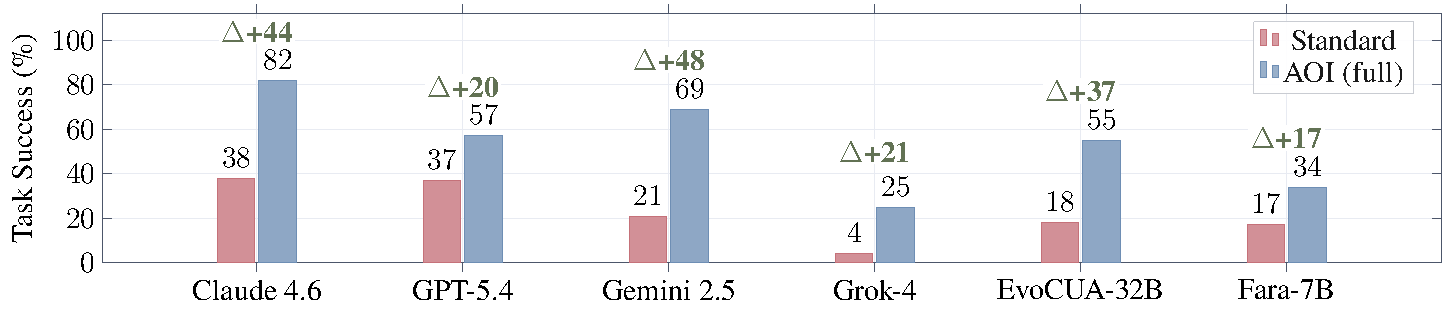
\includegraphics[width=\textwidth]{figures/fig_dynacu_bench_results.pdf}
\caption{\textbf{Main results on DynaCU-Bench (100 tasks).}
AOI substantially improves task success across all evaluated CU models without retraining. Green labels indicate the absolute improvement over the standard screenshot baseline.}
\label{fig:mainresults}
\end{figure*}

Figure~\ref{fig:mainresults} shows the main results.
AOI substantially improves performance across all six models.
For example, on meeting tasks the standard agent often fails because it cannot hear spoken answers, while AOI transcribes the audio and completes the task in far fewer steps. On video and carousel tasks, narration often enables correct answers in a single step.

\emph{Statistical protocol.}
Each configuration is evaluated once on 100 binary tasks. We report paired McNemar exact mid-$p$ tests. Independent seed sweeps later show approximately 3\,pp decoding variability, so small differences should not be over-interpreted.

Figure~\ref{fig:mainresults} shows that AOI improves task success for every model, with gains ranging from +17 to +48 percentage points. Claude Sonnet~4.6 achieves the highest absolute score (82\%), while Gemini~2.5 Flash shows the largest gain (+48\,pp). Open-source models also benefit substantially: EvoCUA-32B improves from 18\% to 55\%, and even the 7B Fara model doubles its success rate (17\%$\rightarrow$34\%). These consistent gains indicate that AOI addresses a perception bottleneck rather than exploiting model-specific behavior.

\textbf{Additional open-source replication (Qwen3-VL family).}
Both Qwen3-VL models reproduce the same trend: the 235B model improves by +42\,pp (22\%$\rightarrow$64\%) and the 30B model by +24\,pp (18\%$\rightarrow$42\%), reinforcing that AOI's gains are model-agnostic.

\begin{table}[t]
\centering
\caption{Open-source replication on DynaCU-Bench (100 tasks) using Qwen3-VL models. Results use the same evaluation protocol as Figure~\ref{fig:mainresults}.}
\label{tab:b1_oss}
\small
\begin{tabular}{@{}l cc cc c@{}}
\toprule
\textbf{Model} & \textbf{Standard} & \textbf{AOI full}
& \textbf{$\Delta$}  & \textbf{$p$ (McNemar)} \\
\midrule
235B-A22B & 22 & \textbf{64} & $+$42 & $4.5\times10^{-10}$ \\
30B-A3B   & 18 & \textbf{42} & $+$24 & $1.8\times10^{-4}$ \\
\bottomrule
\end{tabular}
\end{table}

\textbf{Variance.}
Repeating the headline configuration (Claude~+~AOI~full) across three seeds yields
82\%, 78\%, 76\% (mean 78.7\%, std 3.1\,pp). The reported 82\% thus sits at the upper end of a $\sim$3\,pp decoding variability band.
This quantifies absolute score variance and is complementary to the paired McNemar tests reported above.

\subsection{Per-Family Analysis}

\begin{figure}[t]
\centering
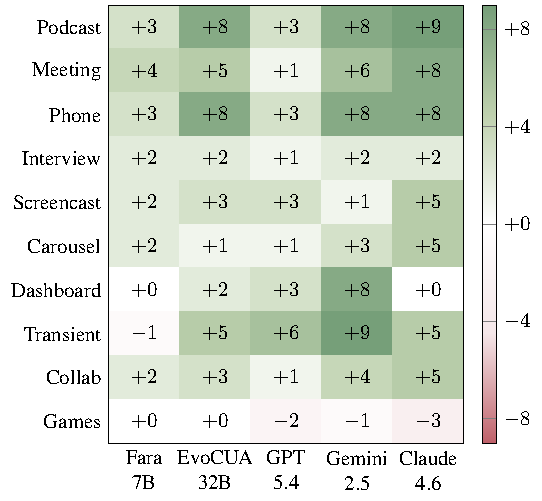
\includegraphics[width=\columnwidth]{figs/fig_heatmap.pdf}
\caption{\textbf{Per-family AOI gain} (AOI full $-$ Standard, tasks per 10) across five models. Families are grouped by modality. Green indicates improvement; red indicates regression.}
\label{fig:heatmap}
\end{figure}

Figure~\ref{fig:heatmap} reveals three patterns. Audio tasks (Podcast, Phone, Meeting) improve the most because they are impossible from screenshots alone. Visual-temporal tasks (Screencast, Carousel, Transient) also improve consistently, whereas Dashboard gains are modest because the relevant information is often visible in a single screenshot. Games is the only family that consistently regresses: it is limited by action latency rather than perception, and AOI's additional observation time exceeds its benefit.

\subsection{Difficulty Breakdown}

AOI improves performance across all difficulty tiers, with the largest absolute gains on medium and hard tasks for stronger models. On Fara-7B, improvements are concentrated on easy tasks, suggesting that reasoning rather than perception is the dominant remaining bottleneck.

\subsection{Efficiency}

Better perception reduces the number of interaction steps enough to outweigh the richer observations, lowering token costs by 15--50\% across cloud models.
Wall-clock time decreases only for the slowest models, where fewer agent steps dominate the added observation overhead. AOI therefore improves cost efficiency while trading off latency on faster models.

% ════════════════════════════════════════════════════════════
\section{Decomposing the Gain}
\label{sec:static}
% ════════════════════════════════════════════════════════════

We decompose AOI's gains in two stages: separating the structured prompt-format effect from genuine perception improvements, then breaking down the perception component channel by channel.

\subsection{Prompt Format vs.\ Perception}
\label{sec:promptperc}

We first rule out the possibility that AOI helps only through prompt reformatting.
\label{sec:static50}\label{sec:structured}\label{sec:promptsub}

\begin{figure}[t]
\centering
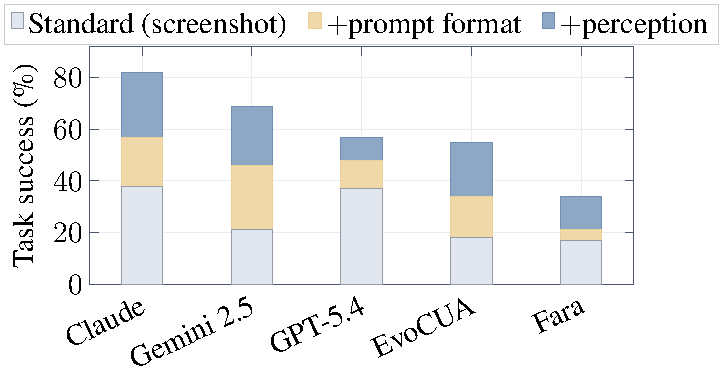
\includegraphics[width=\columnwidth]{figs/fig_decomp.pdf}
\caption{Bars stack the standard screenshot baseline, the gain from the structured observation record alone, and the additional gain from perception (keyframes, audio, and narration).}
\label{fig:decomp}
\end{figure}

On the purely static \textbf{Static-50} benchmark, AOI achieves a perfect 50/50 while the screenshot baseline scores 43/50, demonstrating a beneficial prompt-format effect with no degradation.

On dynamic tasks, a control using only AOI's structured observation record (no keyframes or audio) isolates the prompt-format contribution. Figure~\ref{fig:decomp} shows both prompt-format and perception components are positive for every model. The balance is model-specific: Claude is perception-heavy, Gemini~2.5 is prompt-heavy, and Fara-7B cannot exploit the richer prompt. Within the prompt component, the DOM-element list is the largest lever.

\subsection{Perception Channel Contributions}
\label{sec:analysis}\label{sec:ablation}\label{sec:narration_discard}\label{sec:keyframe_context}

\begin{figure}[t]
\centering
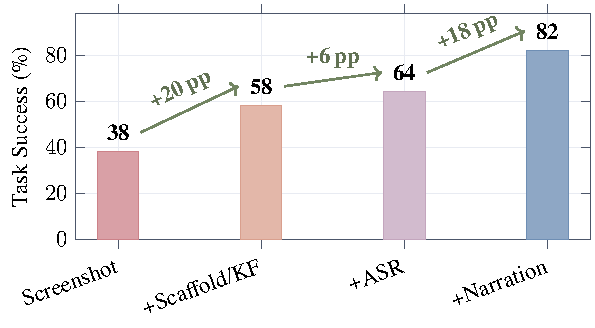
\includegraphics[width=\columnwidth]{figures/fig_component_contribution.pdf}
\caption{Progressive contribution of AOI components on Claude Sonnet~4.6.}
\label{fig:ablation}
\end{figure}

Figure~\ref{fig:ablation} shows incremental gains. Keyframe images add only +1\,pp as raw input but +10\,pp once narrated (Figure~\ref{fig:analysis}b), with benefits concentrated on Transient and Carousel tasks. Keyframe selection strategy has negligible impact (Table~\ref{tab:ablation_stats}). Audio transcription adds directional gains on audio families, while visual narration is the largest single component (+18\,pp).

\begin{table}[!h]
\centering
\caption{Pairwise McNemar exact mid-$p$ tests between successive ablation tiers
on Claude Sonnet~4.6. The selection-method group is statistically indistinguishable, only the between-tier transitions are significant.}
\label{tab:ablation_stats}
\small
\begin{tabular}{@{}l r l@{}}
\toprule
\textbf{Comparison} & \textbf{Total}  & \textbf{$p$} (McNemar) \\
\midrule
Standard $\to$ Uniform 1\,FPS         & 38 / 58 &  $8.8 \times 10^{-5}$ \\
Uniform 1\,FPS $\to$ Uniform 3\,FPS   & 58 / 56 &  $0.77$ \\
Uniform 3\,FPS $\to$ Pixel-diff       & 56 / 58 &  $0.75$ \\
Pixel-diff $\to$ Random keyframes      & 58 / 56 &  $0.69$ \\
Random keyframes $\to$ CLIP adaptive   & 56 / 58 &  $0.75$ \\
CLIP adaptive $\to$ AOI visual+ASR     & 58 / 64 &  $0.18$ \\
AOI visual+ASR $\to$ AOI full          & 64 / 82 &  $5.3 \times 10^{-4}$ \\
\bottomrule
\end{tabular}
\end{table}

\begin{figure}[t]
\centering
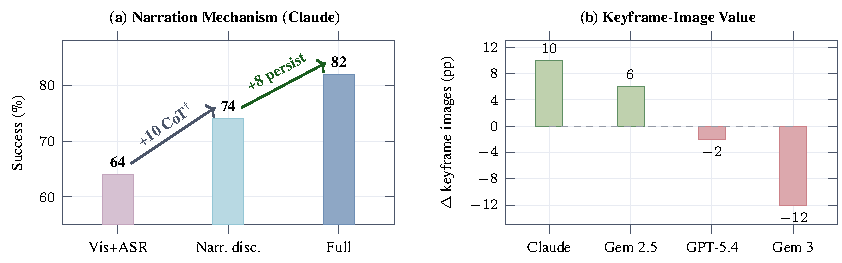
\includegraphics[width=\columnwidth]{figs/fig_analysis.pdf}
\caption{\textbf{Contribution of narration and keyframes.}
\textbf{(a)} Visual narration improves performance, with most of the gain arising from inference-time articulation rather than persistent memory.
\textbf{(b)} The value of keyframes is model-dependent: positive for Claude and Gemini~2.5, neutral for GPT-5.4, and negative for Gemini~3.}
\label{fig:analysis}
\end{figure}

A narration-discarded control (Figure~\ref{fig:analysis}a) attributes most of narration's benefit to inference-time articulation, with persistence mattering mainly on multi-step tasks.

The keyframe channel is the most model-dependent: strongly positive with narration on Claude and Gemini~2.5, but regressing on Gemini~3 due to image-token dilution. Overall, AOI components must be tuned per model.

% ════════════════════════════════════════════════════════════
\section{Model Case Studies: Later-Released Models}
\label{sec:newer}
% ════════════════════════════════════════════════════════════

We evaluated AOI on three additional models released after the main experiments (Table~\ref{tab:newer}).

\label{sec:grok}\label{sec:why_g3}\label{sec:keyframe_probe}\label{sec:diagmap}

\begin{table}[t]
\centering
\caption{Results on later-released models (100 tasks each). Gemini~3~Flash tests whether AOI gains transfer to the next generation, while the Grok rows isolate inference latency.}
\label{tab:newer}
\small
\setlength{\tabcolsep}{4pt}
\begin{tabular}{@{}lcccc@{}}
\toprule
\textbf{Model} & \textbf{Standard} & \textbf{AOI-full}
& \textbf{$\Delta$} & \textbf{$p$ (McNemar)} \\
\midrule
Gemini 3 Flash               & 36     & 45     & $+$9     & 0.18 \\
Grok-4.3                     & 25  & 65  & $+$40  & $8.2\times10^{-10}$ \\
Grok-4-fast-reasoning        & 19  & 47  & $+$28  & $4.9\times10^{-6}$ \\
\bottomrule
\end{tabular}
\end{table}

\textbf{Grok models} are primarily limited by high inference latency rather than perception.
The original Grok-4 achieves only +21\,pp with AOI due to frequent timeouts. A lower-latency variant and the newer Grok-4.3 show substantially stronger performance (+28\,pp and +40\,pp respectively), indicating that reducing latency unlocks much of AOI's potential.

\textbf{Gemini~3~Flash} achieves only a modest +9\,pp net gain. A four-way decomposition (Figure~\ref{fig:gemini3}) reveals a cancellation of effects: audio and the structured scaffold help as usual, but the keyframe stream regresses by $-12$\,pp due to image-token dilution. Dropping keyframes alone recovers +21\,pp over the standard baseline, showing the default AOI bundle is mis-tuned for this model.

\begin{figure}[t]
\centering
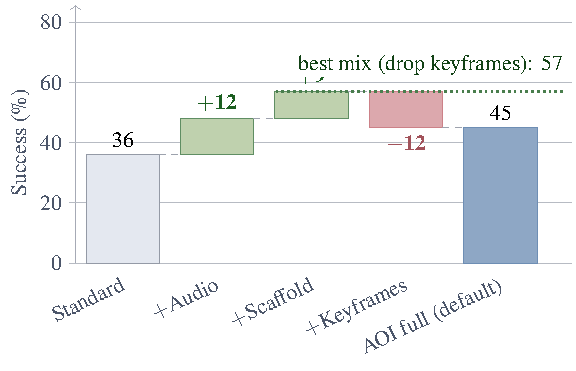
\includegraphics[width=\columnwidth]{figs/fig_gemini3.pdf}
\caption{\textbf{Gemini~3~Flash achieves only a small net gain ($+9$\,pp).} Audio and the structured scaffold remain beneficial, but keyframes reduce performance by $12$\,pp.}
\label{fig:gemini3}
\end{figure}

These cases illustrate that AOI gains are robust but model-specific: the optimal component mix must be chosen per model rather than applied as a fixed bundle.

% ════════════════════════════════════════════════════════════
\section{Comparison with Streaming Multimodal Baselines}
\label{sec:streaming}
% ════════════════════════════════════════════════════════════

A natural alternative is a \emph{streaming multimodal model} that integrates perception and reasoning, such as Gemini Live~\citep{geminilive} or the OpenAI Realtime API~\citep{openairealtime}.
Neither is a computer-use agent, so we adapt both to DynaCU-Bench by streaming page audio and screenshots into a single session and executing returned tool calls. We evaluate the highest vision- and function-calling-capable tier of each on the same 12-task audio subset used for AOI.

\begin{table}[t]
\centering
\caption{Streaming multimodal baselines vs. AOI on a 12-task audio subset (3 tasks each from Podcast, Meeting, Phone, and Interview).}
\label{tab:streaming}
\small
\setlength{\tabcolsep}{4.5pt}
\begin{tabular}{@{}l cccc c@{}}
\toprule
\textbf{Configuration} & \textbf{Pod} & \textbf{Meet} & \textbf{Phone} & \textbf{Intv} & \textbf{Total / 12} \\
\midrule
OpenAI Realtime          & 0 & 0 & 0 & 3 & 3 \scriptsize(25\%) \\
Gemini Live              & 0 & 0 & 0 & 0 & 0 \scriptsize(0\%) \\
\rowcolor{bestcolor}
AOI~full (Claude 4.6)    & 3 & 3 & 3 & 3 & \textbf{12} \scriptsize(100\%) \\
\bottomrule
\end{tabular}
\end{table}

Both underperform the AOI by a wide margin (Table~\ref{tab:streaming}).
OpenAI Realtime succeeds only on interview questions answerable from a single audio chunk, while Gemini Live rarely emits usable tool calls.
A sanity check on five purely visual tasks confirms the adapters function correctly: both baselines execute valid browser actions (5/5) but solve none of the tasks, whereas AOI-equipped Claude solves 4/5.
Streaming multimodal interaction alone is therefore insufficient; the critical capability is persisting transient observations as text that can guide future actions.

% ════════════════════════════════════════════════════════════
\section{Related Work}
\label{sec:related}
% ════════════════════════════════════════════════════════════

\textbf{Interface Design over Model Training.}
Much agent progress comes from redesigning the agent--computer interface rather than the model weights. Action interfaces have evolved through richer command sets~\citep{sweagent}, executable code actions~\citep{codeact}, and element-grounded actions~\citep{mind2web}.
Observation interfaces have instead focused on enriching individual screenshots with accessibility trees, HTML surrogates, and overlays~\citep{webarena,mind2web,setofmark,seeact}. None addresses temporal or multimodal observation.

\textbf{Computer-Use Agents.}
Recent CU agents span closed-source systems~\citep{anthropic2024claude,openai2025cua,gemini25cu,surfer2} and open-source models~\citep{uitars2,opencua,fara7b,guiowl,coact}, with
Agent~S3~\citep{agents3} demonstrates competitive open-source performance.
Existing surveys~\citep{cusurvey} discuss many challenges but not observation as a distinct design axis; all current agents retain the screenshot-per-step loop.

\textbf{Streaming Multimodal Models.}
Gemini Live~\citep{geminilive} and OpenAI Realtime~\citep{openairealtime} process continuous streams but bundle perception and reasoning in one model. Section~\ref{sec:streaming} shows they underperform AOI on grounded computer-use tasks. Our work is complementary: AOI provides a modular perception layer usable by any CU model.

\textbf{Video and GUI Understanding.}
Benchmarks such as GUI-World~\citep{guiworld}, VideoWebArena~\citep{videowebarena}, CUA-Suite~\citep{cuasuite}, and MemGUI-Bench~\citep{memguibench} expose the limitations of static observation and GUI memory, but do not provide observation mechanisms compatible with existing CU agents.

\textbf{Keyframe selection.}
Prior work studies CLIP-based frame selection and sampling for offline video QA~\citep{videotree,aks,apollo}. In contrast, AOI performs real-time observation filtering for interactive computer use, combining a sub-millisecond pixel gate with CLIP only on changed frames.

\textbf{Adaptive middleware for GUI agents.}
Cradle~\citep{cradle}, ScreenLLM~\citep{screenllm}, StreamAgent~\citep{streamagent}, and Dispider~\citep{dispider} separate or adapt perception, but none combines adaptive observation, audio, and persistent multimodal memory for computer-use agents.

\textbf{Structured agent interfaces.}
Protocols such as MCP~\citep{mcp} and NLWeb~\citep{nlweb} bypass perception through structured APIs. They require website cooperation, whereas AOI operates on arbitrary unmodified interfaces.

% ════════════════════════════════════════════════════════════
\section{Limitations}
\label{sec:limitations}
% ════════════════════════════════════════════════════════════

\textbf{Latency and temporal resolution.}
AOI extends perception but not decision speed: CU models still require 1--5\,s per
step and the screen is sampled at ${\sim}3$\,Hz, placing sub-${\sim}300$\,ms events
and real-time games outside its scope.

\textbf{Perception is not reasoning.}
Better observations do not improve reasoning; on smaller models, reasoning capacity
remains the primary bottleneck.

\textbf{Audio is speech-only and narration can err.}
AOI transcribes speech but not non-speech sounds, and visual narrations can
propagate recognition errors through the trajectory.

\textbf{External validity.}
Experiments use a controlled browser with synthesized audio. Evaluating AOI on
existing dynamic-GUI benchmarks requires re-instrumenting each benchmark's
interaction harness and remains future work.

\textbf{Statistical power.}
Each configuration is evaluated once on 100 tasks. Paired McNemar tests support
comparisons, but differences of only a few percentage points should not be
over-interpreted.

% ════════════════════════════════════════════════════════════
\section{Conclusion}
\label{sec:conclusion}
% ════════════════════════════════════════════════════════════

Computer-use agents are blind between screenshots and deaf to audio because
observation is tied to action: one screenshot per step.
We argued the \emph{observation} is a separable design axis and introduced the AOI, a perception layer that is transparent on static work, adaptive on dynamic content, and compatible with existing CU models without retraining. Across eight models, AOI turns many dynamic tasks that are nearly impossible from screenshots into solvable ones while reducing token cost.

Our analysis further shows that keyframe selection alone contributes little: gains emerge when observations are converted into persistent text, and the best observation recipe is model-dependent rather than universal. We release the AOI and DynaCU-Bench to support future research on observation interfaces for computer-use agents.

% ════════════════════════════════════════════════════════════
\bibliography{references}
\end{document}
